\documentclass[]{scrartcl}

% Поддержка русского языка
\usepackage[utf8]{inputenc}
\usepackage[russian]{babel}
\usepackage{setspace,amsmath}

%opening
\title{Компиляция и исполнение Java приложений под капотом}
\author{Голов Павел}

% Настройки полей документа
\usepackage{indentfirst}

% Графические пакеты
\usepackage{graphicx}
\graphicspath{{img/}}

% Пакет для отображения кода
\usepackage{listings}

\begin{document}

\maketitle

\begin{center}
	Статья на конкурс для сайта JavaRush.
\end{center}

\thispagestyle{empty}

\newpage

\section{Вступление}

\begin{figure}[h]
	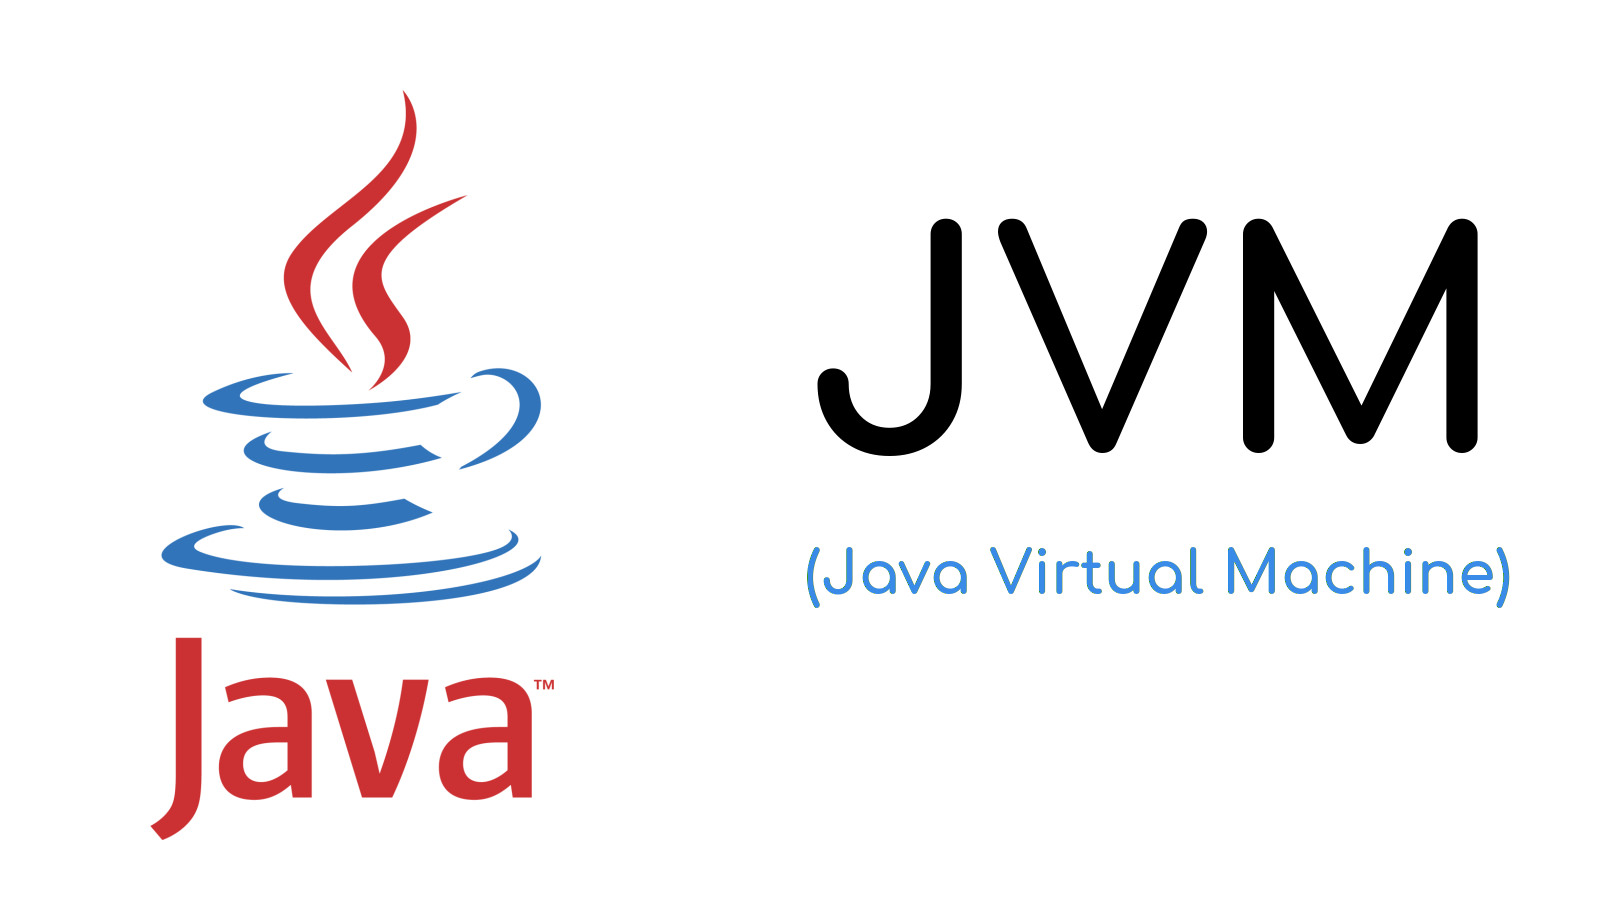
\includegraphics[width=\linewidth]{JVM.jpg}
\end{figure}

Всем привет! Сегодня я хотел бы поделиться знаниями о том, что происходит под капотом JVM (Java Virtual Machine) после того, как мы запускаем написанное Java приложение. В наше время существуют моднейшие среды разработки, которые помогают не думать о внутреннем устройстве JVM, компиляции и выполнении Java - кода, из за чего новые разработчики могут упустить эти важные аспекты. В то же время, на собеседованиях часто задают вопросы касательно этой темы,  из-за чего я и решил написать статью.

\section{Основная часть}

\subsection{Компиляция в байт-код}

\begin{figure}[h]
	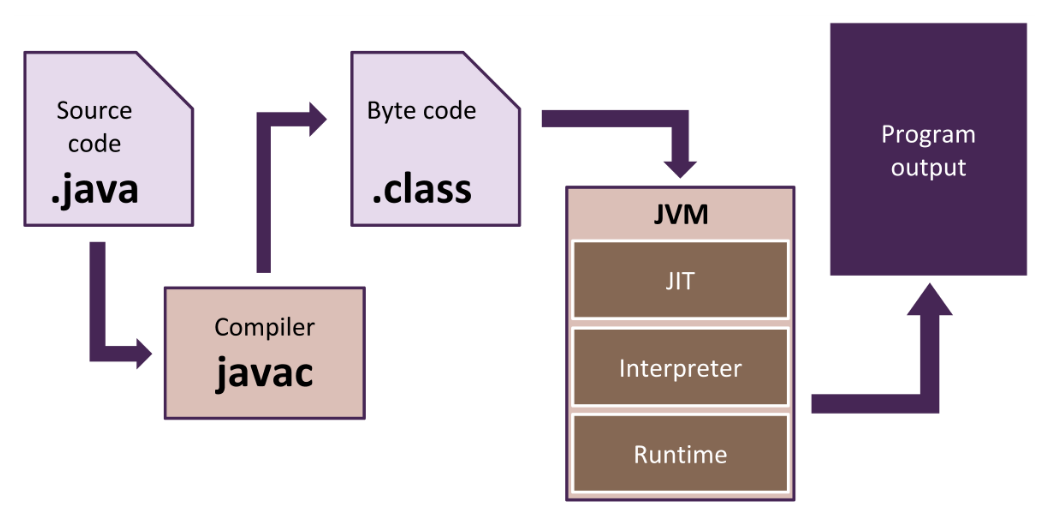
\includegraphics[width=\linewidth]{from-source-to-program.png}
	\caption{От компиляции до исполнения программы}
\end{figure}


Начнем с теории. Когда мы пишем какое-либо приложение, мы создаем файл с расширением .java и помещаем в него код на языке программирования Java. Такой файл, содержащий код, понятный человеку, называется файлом с исходным кодом. После того, как файл с исходным кодом готов, нужно его выполнить! Но на данной стадии в нем содержится информация, понятная только человеку. 

Java - мультиплатформенный язык программирования. Это значит, что программы, написанные на языке Java, можно выполнять на любой платформе, где установлена специальная исполняющая система Java. Такая система называется Java Virtual Machine (JVM). Для того, чтобы перевести программу из исходного кода в код, понятный JVM, нужно её скомпилировать. Код, понятный JVM называется байт-кодом и содержит набор инструкций, которые в дальнейшем будет исполнять виртуальная машина.

Для компиляции исходного кода в байт-код существует компилятор javac, входящий в поставку JDK (Java Development Kit). На вход компилятор принимает файл с расширением .java, содежащий исходный код программы, а на выходе выдает файл с расширением .class, содержащий байт-код, необходимый для исполнения программы виртуальной машиной.

После того, как программа была скомпилирована в байт код, она может быть выполнена с помощью виртуальной машины.

\subsection{Пример компиляции и выполнения программы}

Предположим, что у нас есть простая программа, содержащаяся в файле Calculator.java, которая принимает 2 численных аргумента командной строки и печатает результат их сложения:

\begin{lstlisting}
class Calculator {
	public static void main(String[] args){
		int a = Integer.valueOf(args[0]);
		int b = Integer.valueOf(args[1]);

		System.out.println(a + b);
	}
}
\end{lstlisting}

Для того, чтобы скомпилировать эту программу в байт код, воспользуемся компилятором javac в командной строке:

\begin{lstlisting}
javac Calculator.java
\end{lstlisting}

После компиляции на выходе мы получаем файл с байт-кодом Calculator.class, который мы можем исполнить при помощи установленной на нашем компьютере java-машины при помощи команды java в командной строке:

\begin{lstlisting}
java Calculator 1 2
\end{lstlisting}

Заметим, что после названия файла были указаны 2 аргумента командной строки - числа 1 и 2. После выполнения программы, в командной строке выведется число 3.

\subsection{Выполнение программы виртуальной машиной}

Итак, мы запустили написанную программу. Но что же происходит в момент запуска скомпилированной программы виртуальной машиной?

Для начала разберемся, что означают понятия компиляции и интерпретации кода.

Компиляция — трансляция программы, составленной на исходном языке высокого уровня, в эквивалентную программу на низкоуровневом языке, близком машинному коду. 

Интерпретация — пооператорный (покомандный, построчный) анализ, обработка и тут же выполнение исходной программы или запроса (в отличие от компиляции, при которой программа транслируется без её выполнения).

Язык java обладает как компилятором (javac), так и интерпретатором, в роли которого выступает виртуальная машина, которая построчно преобразует байт-код в машинный код и тут же его исполняет. 

Таким образом, когда мы запускаем скомпилированную программу, виртуальная машина начинает её интерпретацию, то есть построчное преобразование байт-кода в машинный код, а так же его исполнение.

К сожалению, чистая интерпретация байт-кода является довольно долгим процессом и делает язык java медленным в сравнении с его конкурентами. Дабы избежать этого, был введен механизм, позволяющий ускорить интерпретацию байт-кода виртуальной машиной. Этот механизм называется Just-in-time компиляцией (JITC).

\subsection{Just-in-time (JIT) компиляция}

Простыми словами, механизм Just-In-Time компиляции заключается в следующем: если в программе присутствуют части кода, которые выполняются много раз, то их можно скомпилировать один раз в машинный код, чтобы в будущем ускорить их выполнение. После компиляции такой части программы в машинный код, при каждом следующем вызове этой части программы виртуальная машина будет сразу выполнять скомпилированный машинный код, а не интерпретировать его, что естественно ускорит выполнение программы.

Ускорение работы программы достигается за счет увеличения потребления памяти (где-то же нам нужно хранить скомпилированный машинный код!) и за счет увеличения временных затрат на компиляцию во время исполнения программы.

JIT компиляция - довольно сложный механизм, поэтому пройдемся по верхам. Всего существует 4 уровня JIT компиляции байт-кода в машинный код. Чем выше уровень компиляции, тем он сложнее, но и одновременно выполнение такого участка будет быстрее, чем участка с меньшим уровнем. JIT - компилятор самостоятельно решает, какой уровень компиляции задать для каждого фрагмента программы на основе того, как часто выполняется этот фрагмент. Под капотом JVM использует 2 JIT - компилятора - C1 и C2. C1 компилятор так же называется клиентским компилятором и способен скомпилировать код только до 3-его уровня. За 4-ый, самый сложны и быстрый уровень компиляции отвечает компилятор C2.

\begin{figure}[h!]
	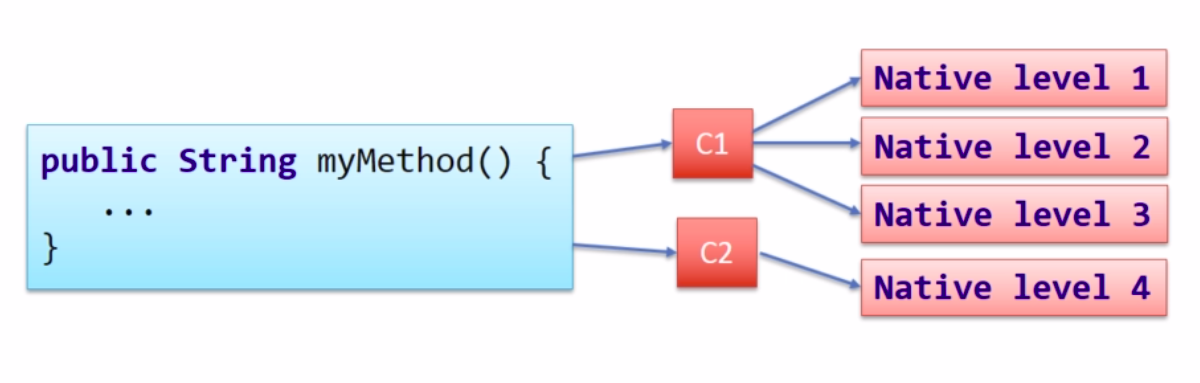
\includegraphics[width=\linewidth]{JIT.png}
	\caption{JIT-компиляция}
\end{figure}

Из вышесказанного можно сделать вывод о том, что для простых, клиентских приложений, выгоднее использовать компилятор C1, так как в этом случае нам важно как быстро стартует приложение. Серверные, долгоживущие приложения могут стартовать большее количество времени, однако в дальнейшем должны работать и выполнять свою функцию быстро - тут нам подойдет компилятор C2.

При запуске Java - программы на x32 версии JVM мы в ручную можем указать, какой режим мы хотим использовать, при помощи флагов -client и -server. При указании флага -client JVM не будет производить сложные оптимизации с байт-кодом, что ускорит время старта приложения и уменьшит количество потребляемой памяти. При указании флага -server приложение будет стартовать большее количество времени из-за сложных оптимизаций байт-кода и будет использовать больше памяти для хранения машинного кода, однако в дальнейшем работать такая программа будет быстрее. В x64 версии JVM флаг -client игнорируется и по умолчанию используется серверная конфигурация приложения.

\section{Заключение}

Вот и подошел к концу мой краткий обзор того, как работает компиляция и исполнение Java-приложения. 

Основные поинты:

1. Компилятор javac преобразует исходный код программы в байт-код, который может быть выполнен на любой платформе, на которой установлена виртуальная машина Java;

2. После компиляции JVM интерпретирует получившийся байт-код;

3. Для ускорения работы Java-приложений, JVM использует механизм Just-In-Time компиляции, который преобразует наиболее часто выполняемые участки программы в машинный код и хранит их в памяти.

Я надеюсь, что эта статья помогла вам более глубоко понять как устроен наш любимый языка программирования. Спасибо за прочтение, критика приветствуется!

\end{document}
